\section{Small stereo roads}
\label{sec:stereoroads}

Proposal and performance of small stereo roads.

\begin{figure}[!htpb]
  \begin{center}
    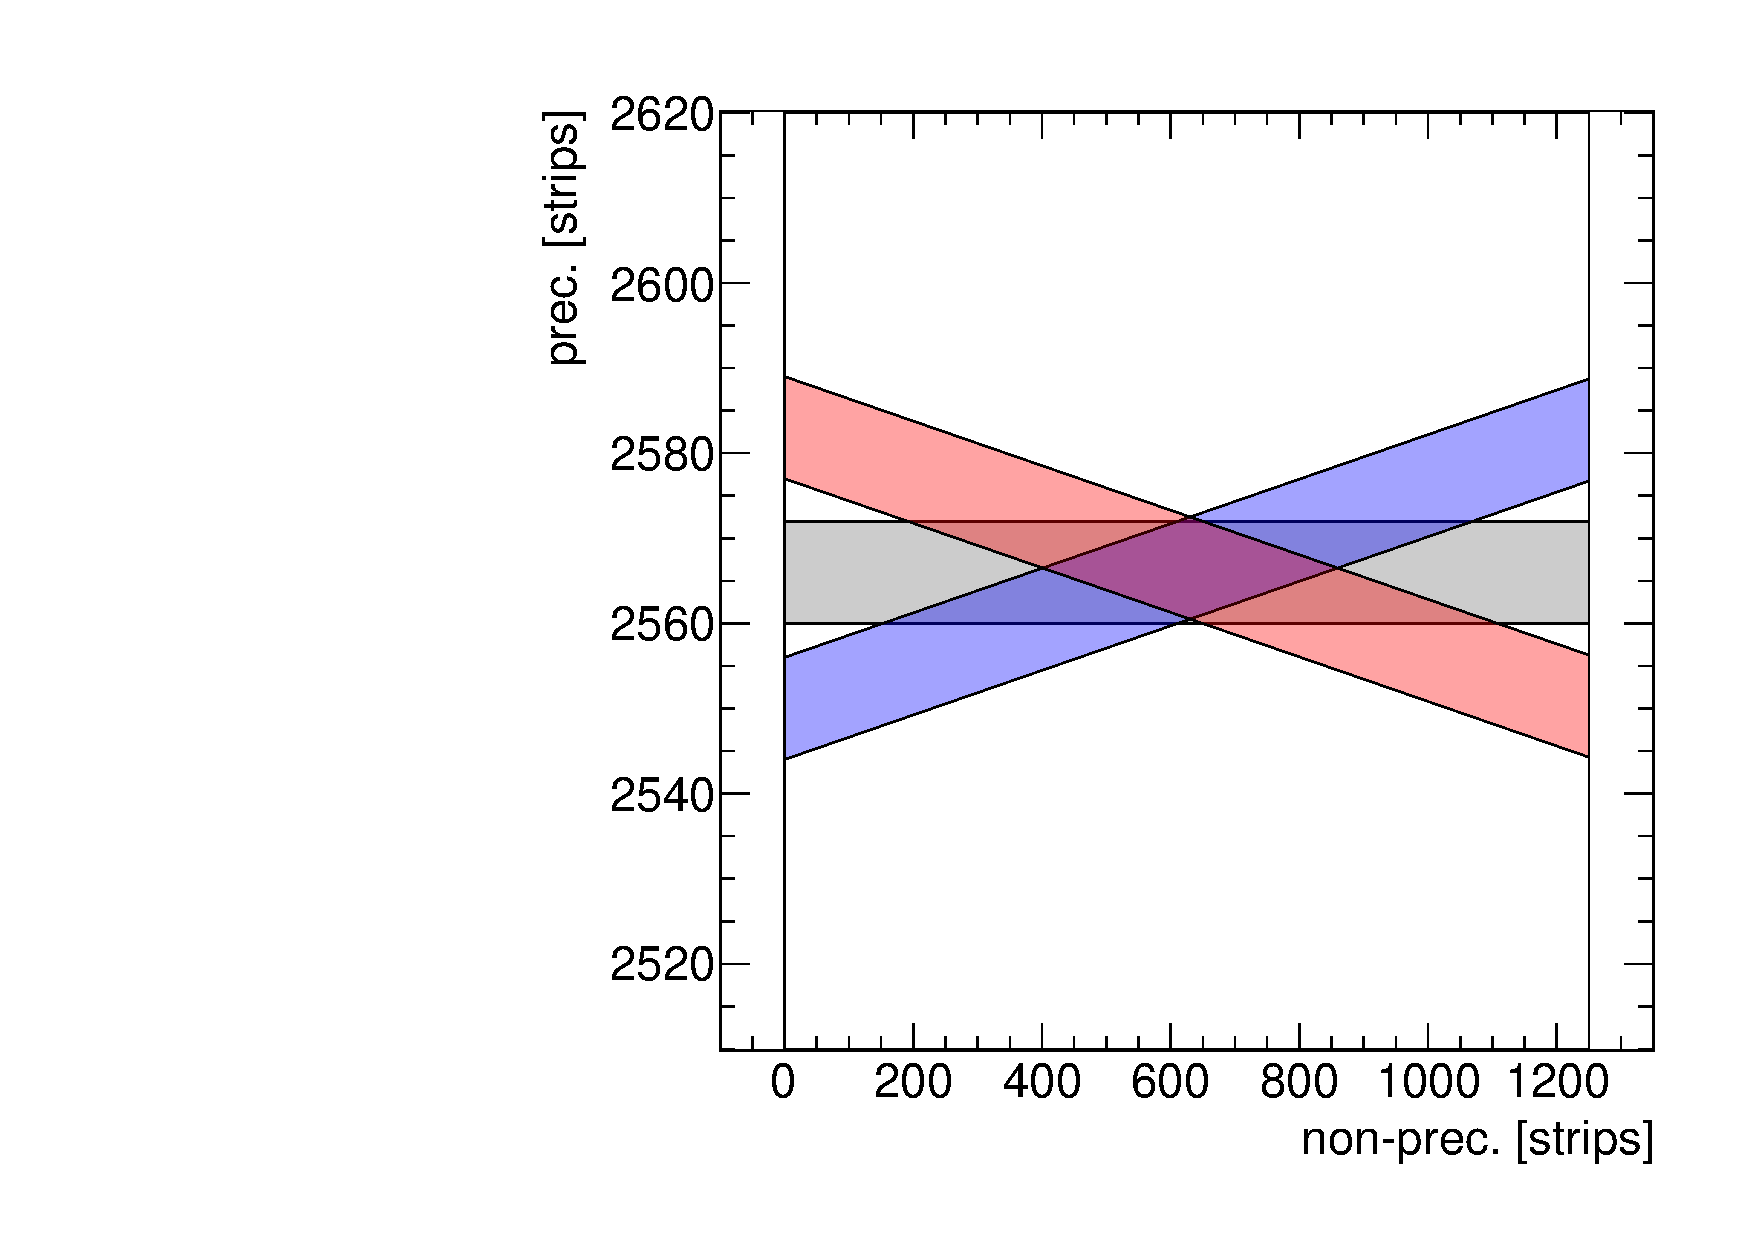
\includegraphics[width=0.48\textwidth]{figures/cartoon_roads_small_smallstereo_1.pdf}
    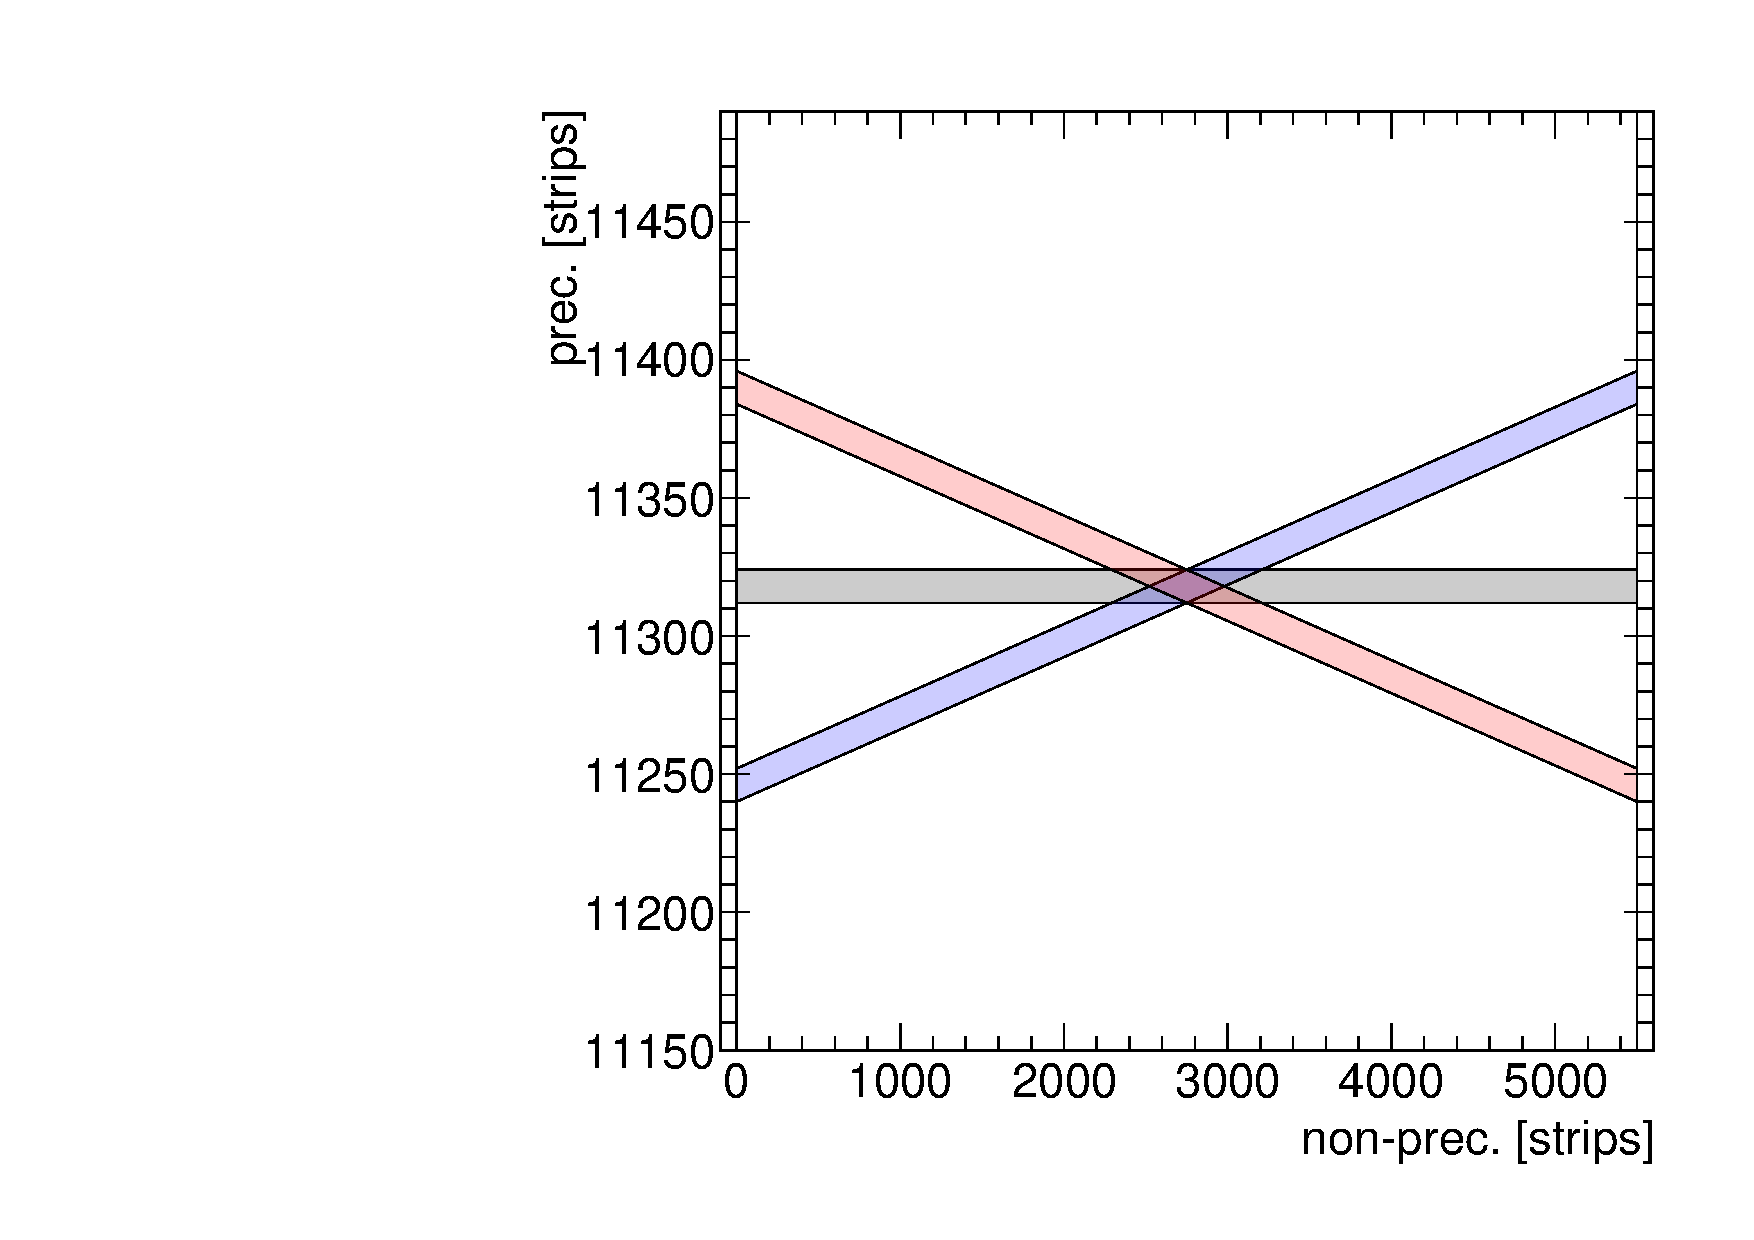
\includegraphics[width=0.48\textwidth]{figures/cartoon_roads_large_smallstereo_1.pdf}
  \end{center}
  \vspace{-10pt}
  \caption{Sketch of the road coverage of the proposed MMTP algorithm, for a small chamber closest to the beamline (left) and large chamber farthest from the beamline (right). The $X$ road is horizontal, the $U$ road is pink and slanted, and the $V$ road is blue and slanted. For ease of digestion, only one pair of $U$ and $V$ roads are shown, and they do not cover the entire $X$ road.}
  \label{fig:cartoon_smallroads_1}
\end{figure}

\begin{figure}[!htpb]
  \begin{center}
    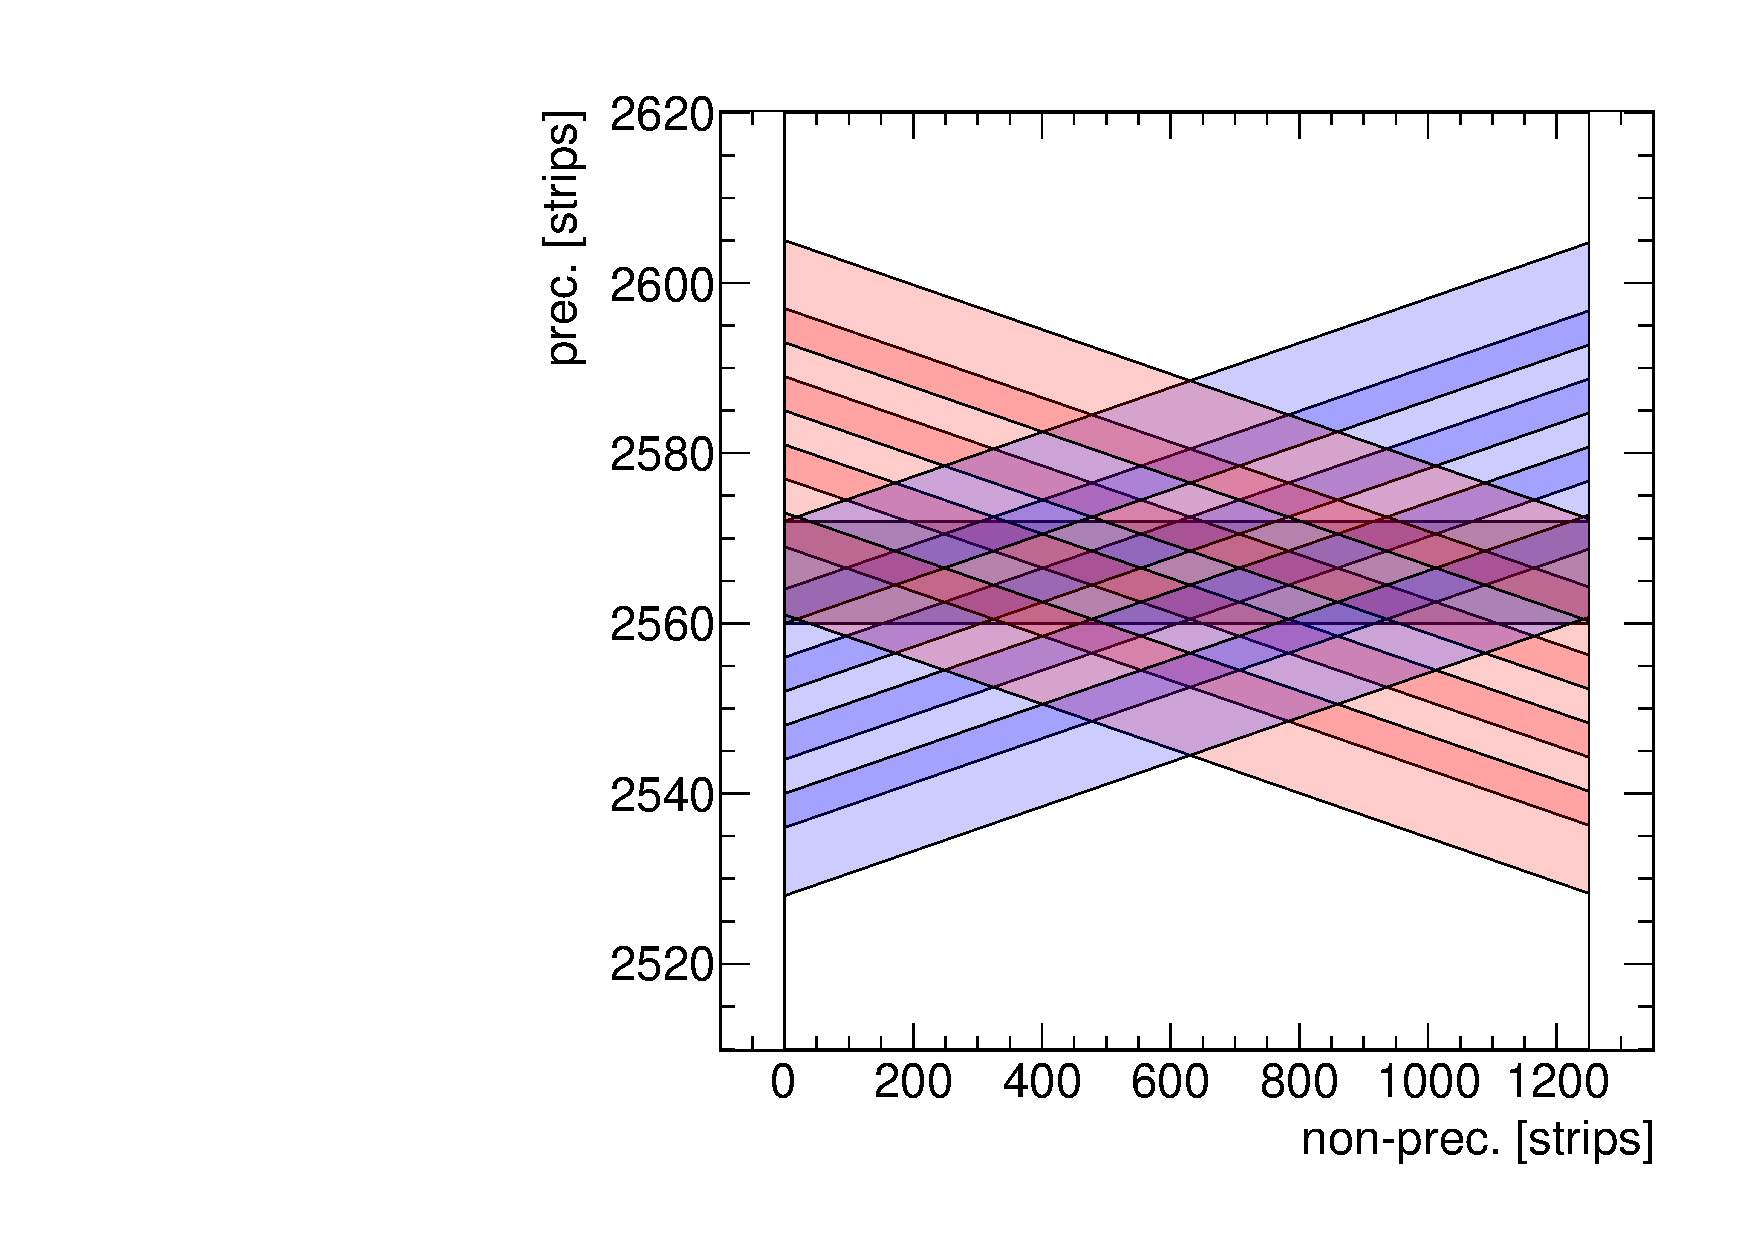
\includegraphics[width=0.48\textwidth]{figures/cartoon_roads_small_smallstereo_N.pdf}
    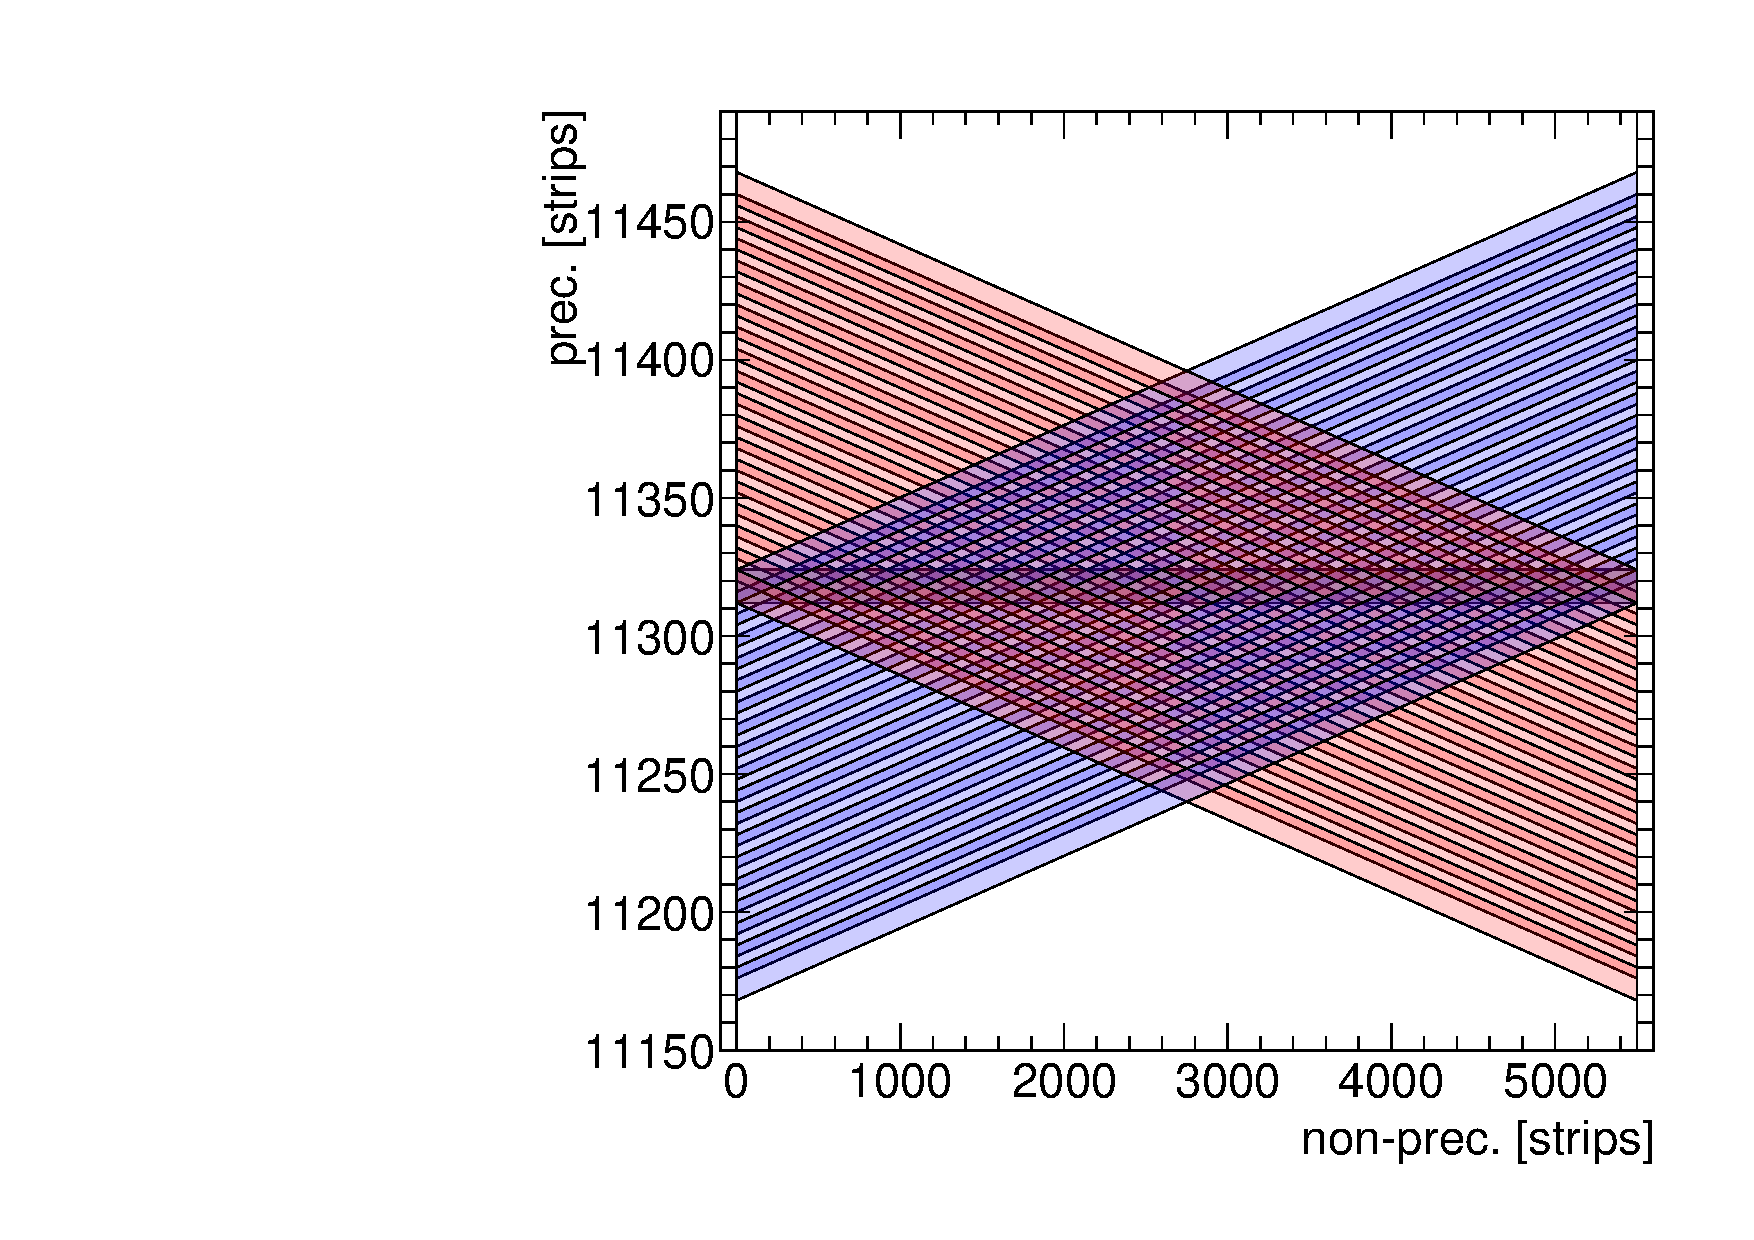
\includegraphics[width=0.48\textwidth]{figures/cartoon_roads_large_smallstereo_N.pdf}
  \end{center}
  \vspace{-10pt}
  \caption{Sketch of the road coverage of the proposed MMTP algorithm, for a small chamber closest to the beamline (left) and large chamber farthest from the beamline (right). The $X$ road is horizontal, the $U$ roads are pink and slanted, and the $V$ roads are blue and slanted. The small chamber requires five pairs of $U$ and $V$ roads to cover one $X$ road, and the large chamber requires 19.}
  \label{fig:cartoon_smallroads_N}
\end{figure}

\begin{figure}[!htpb]
  \begin{center}
    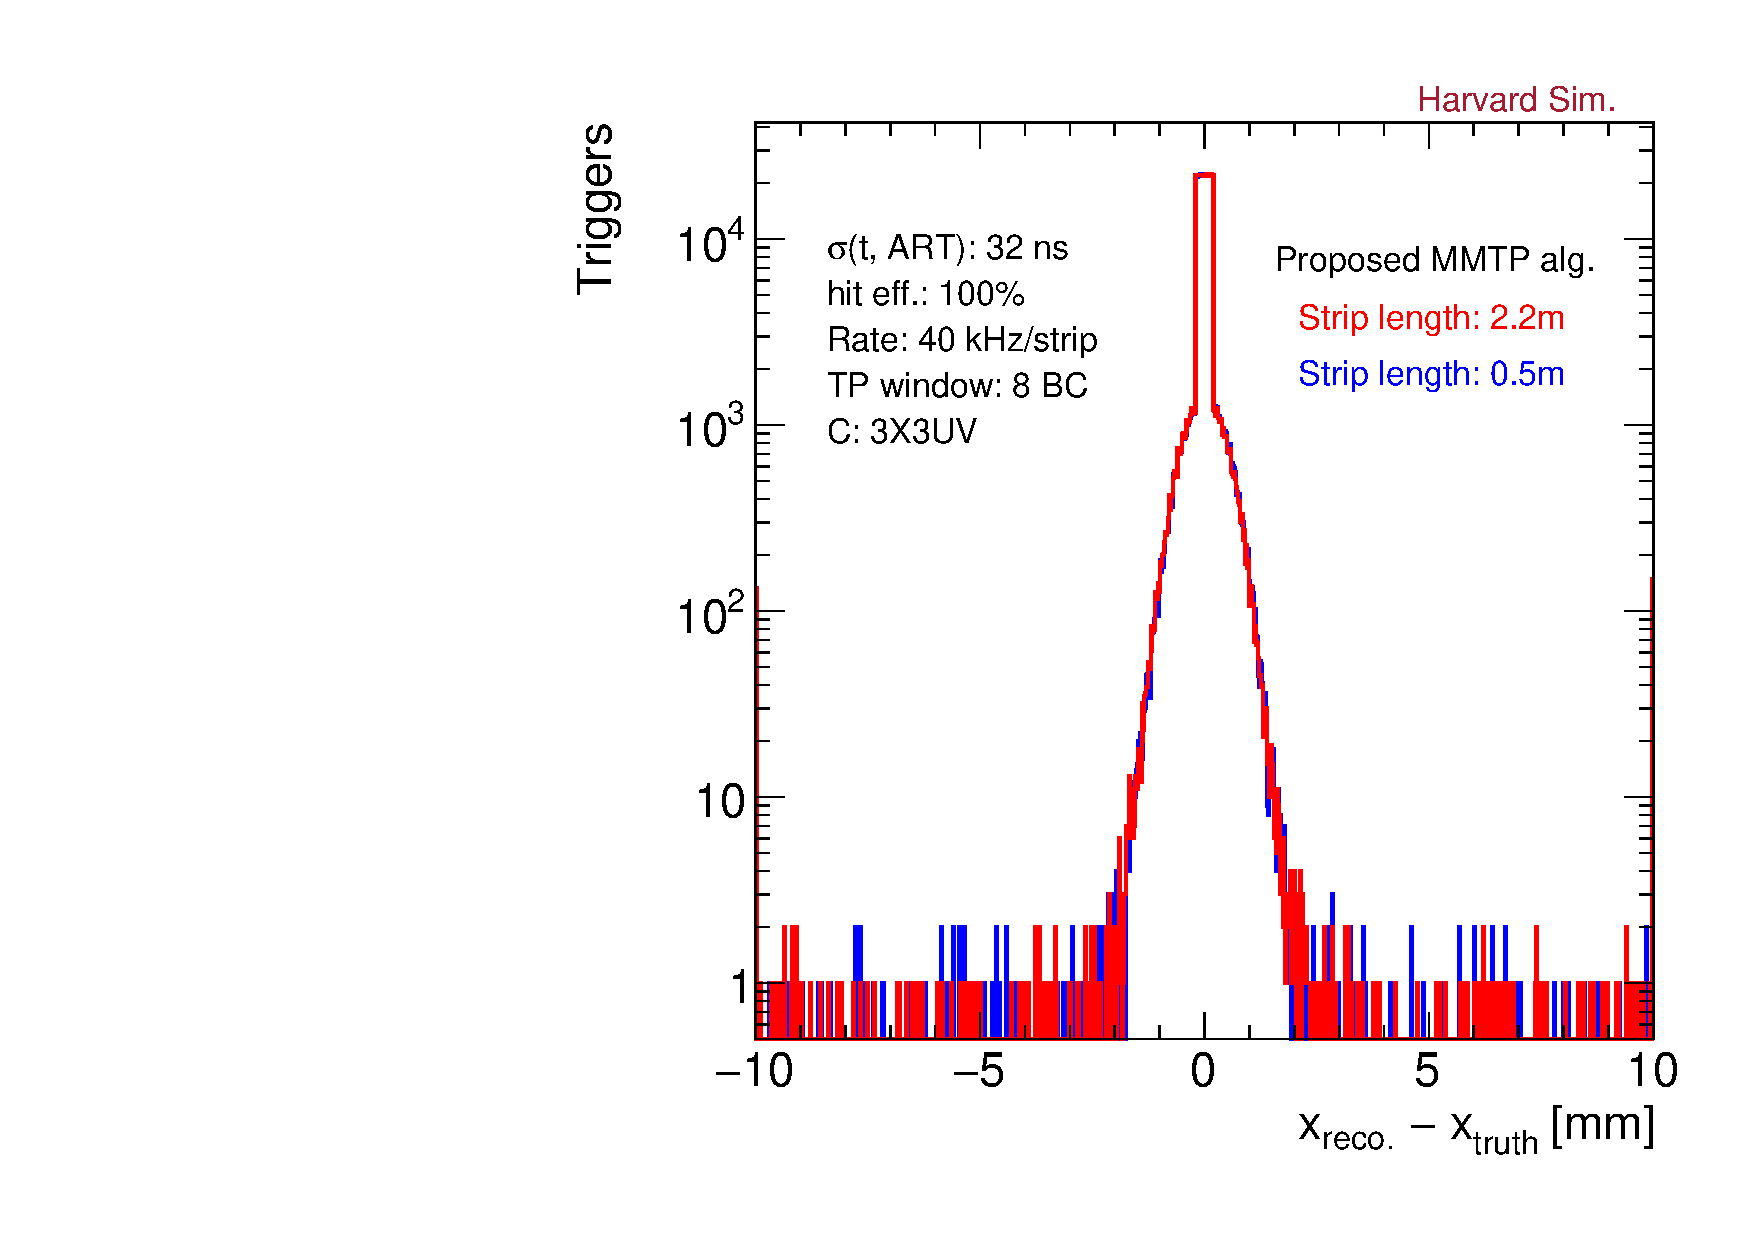
\includegraphics[width=0.48\textwidth]{figures/xres_new.pdf}
    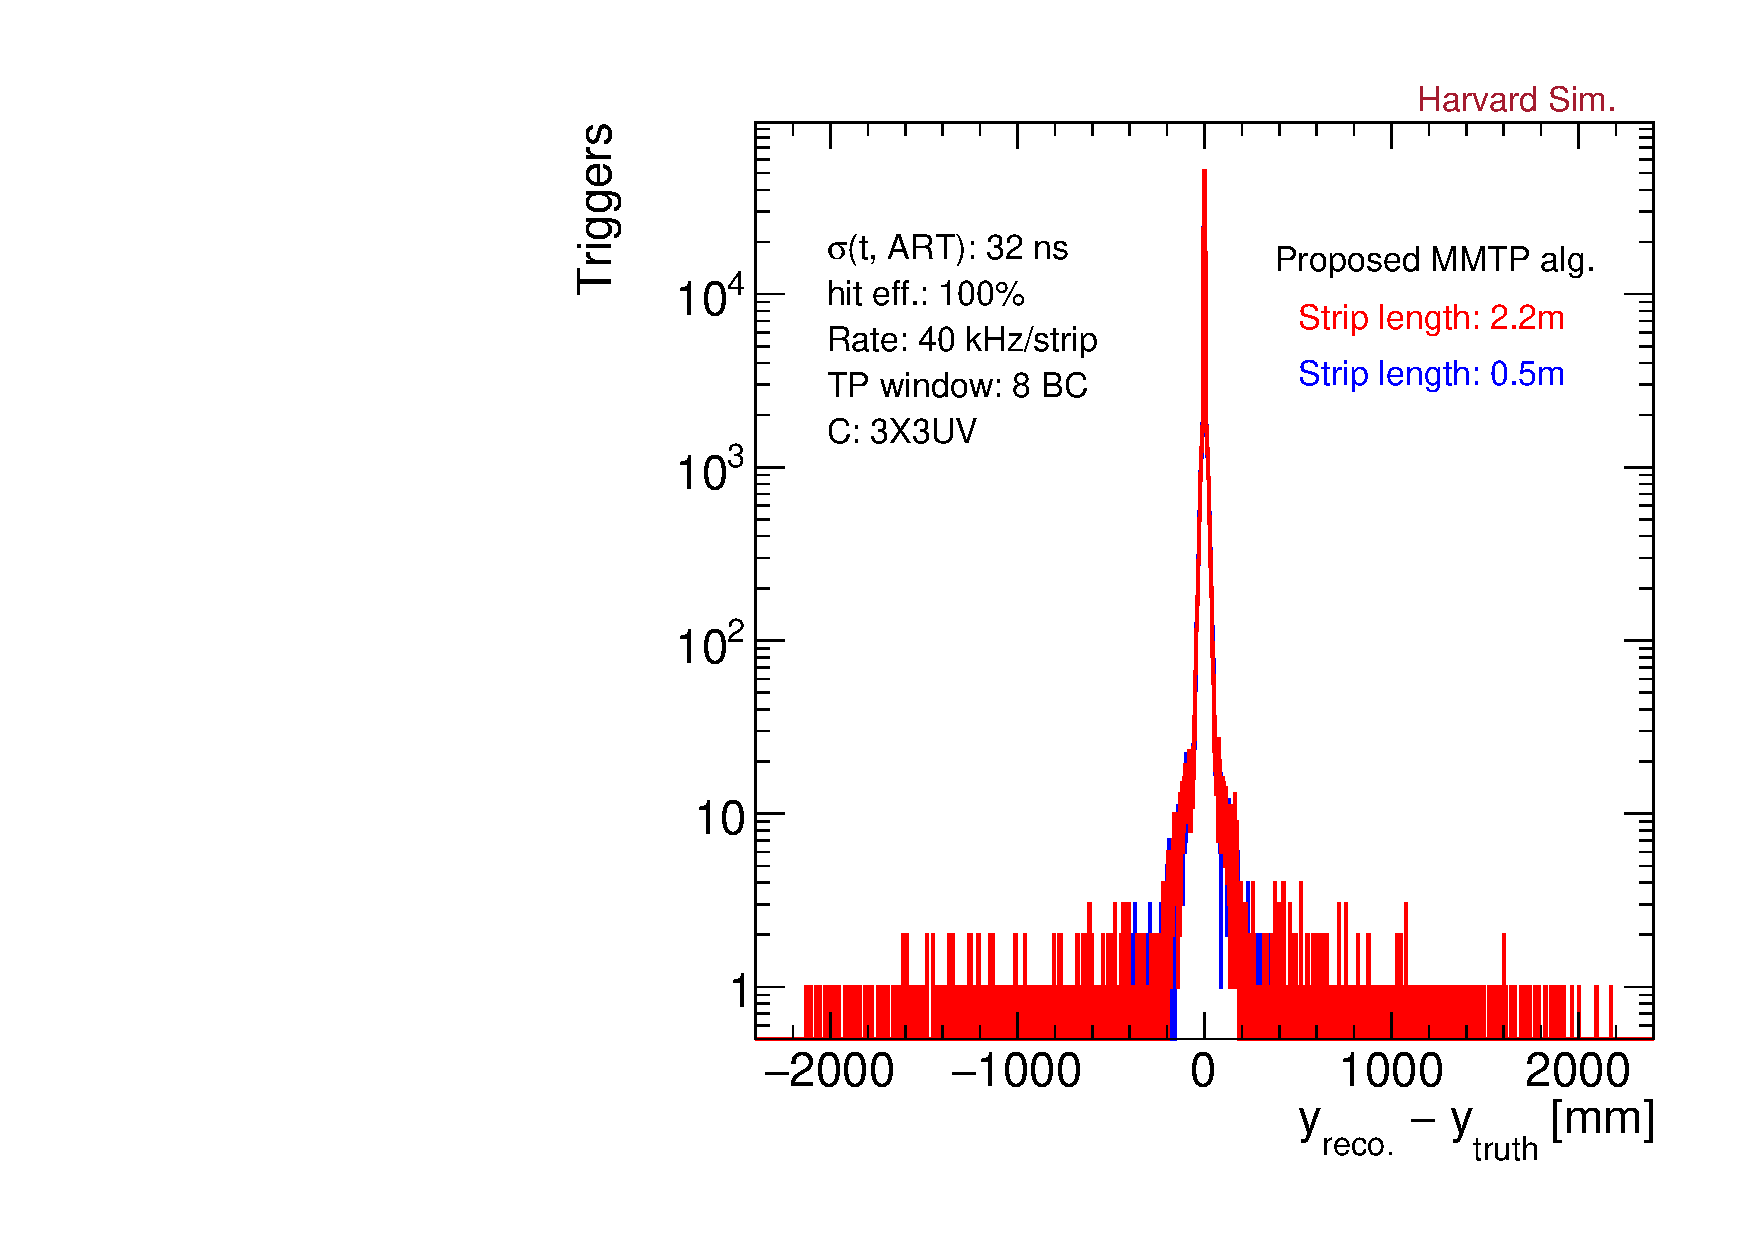
\includegraphics[width=0.48\textwidth]{figures/yres_new.pdf}
    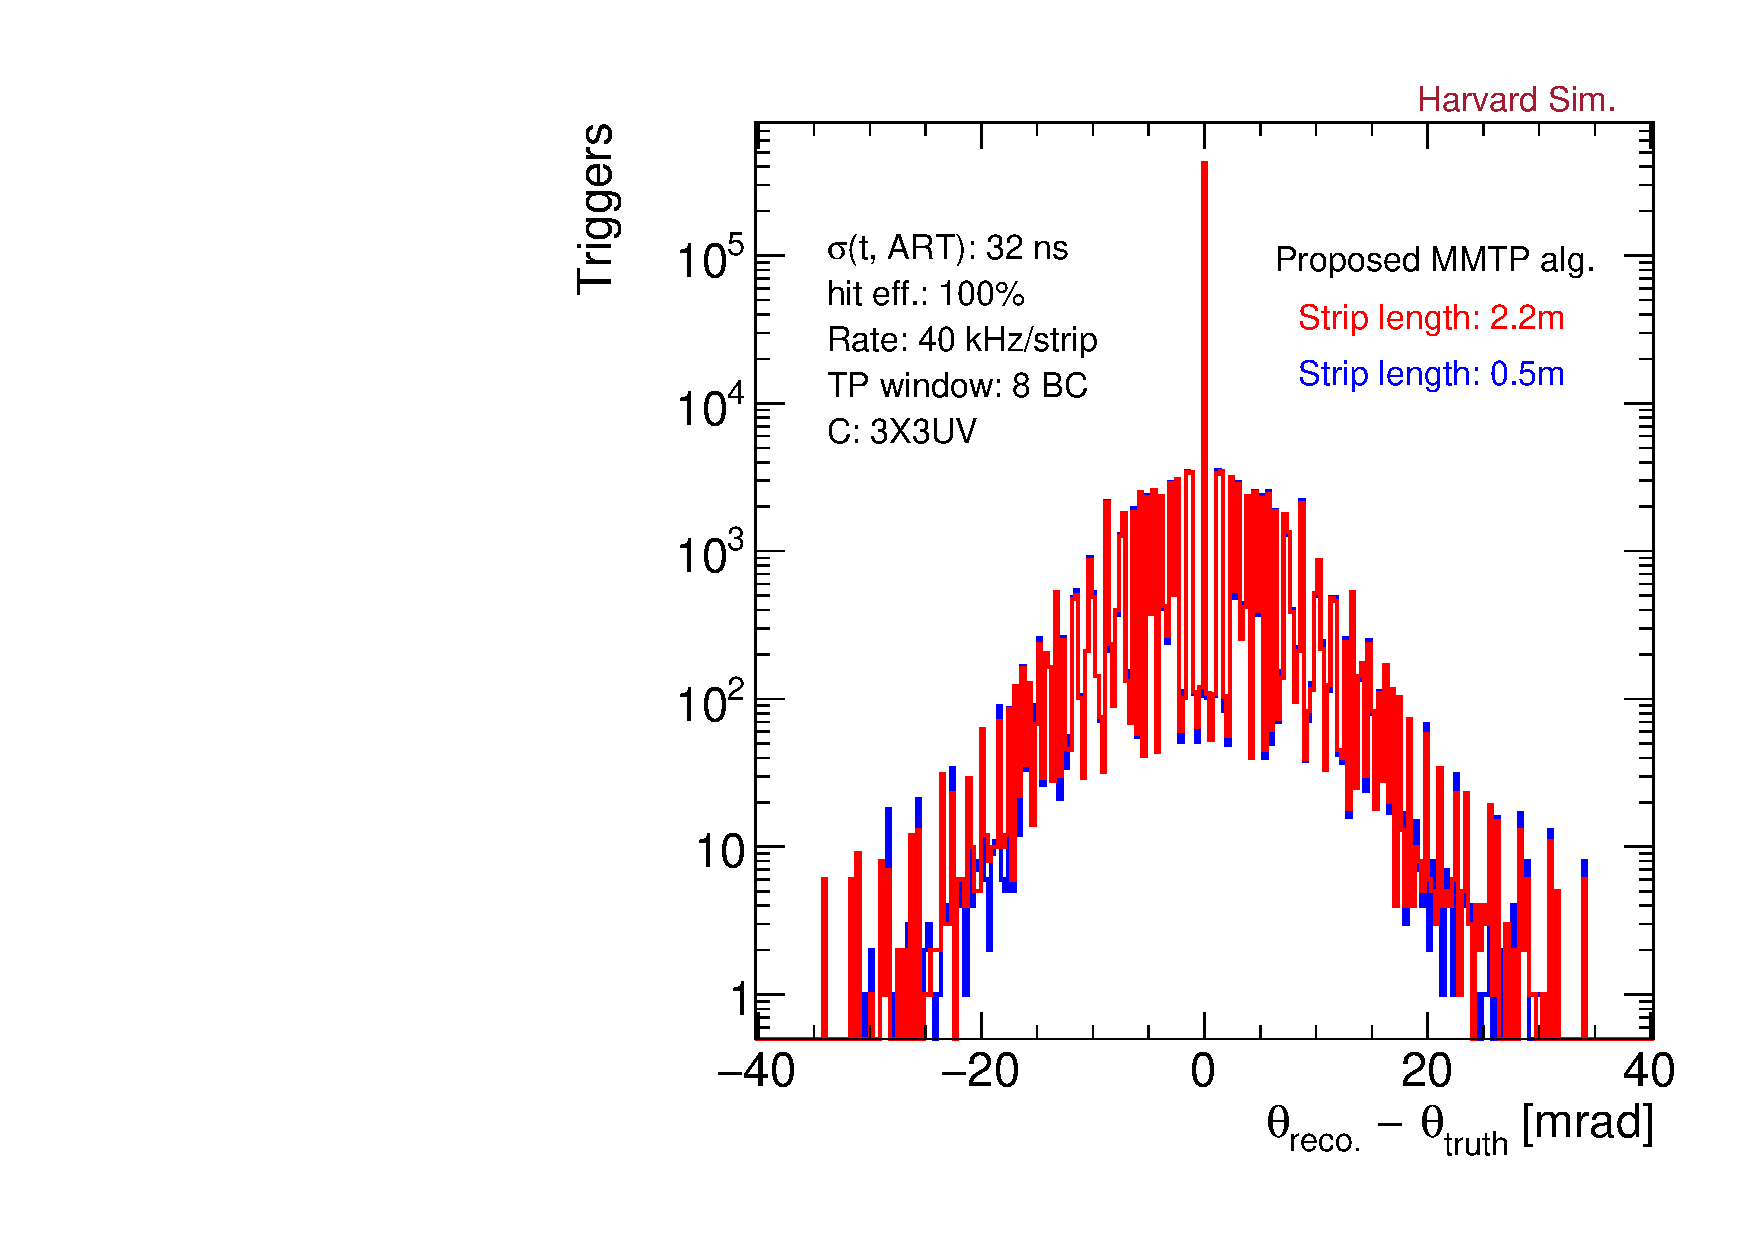
\includegraphics[width=0.48\textwidth]{figures/mres_new.pdf}
  \end{center}
  \vspace{-10pt}
  \caption{Distribution of $x_\text{reco.} - x_\text{truth}$ (top, left), $y_\text{reco.} - y_\text{truth}$ (top, right) and $\theta_\text{reco.} - \theta_\text{truth}$ (bottom) for the nominal MMTP algorithm with uncorrelated background at a rate of 40 kHz per strip.}
  \label{fig:resolutions_old}
\end{figure}

\begin{figure}[!htpb]
  \begin{center}
    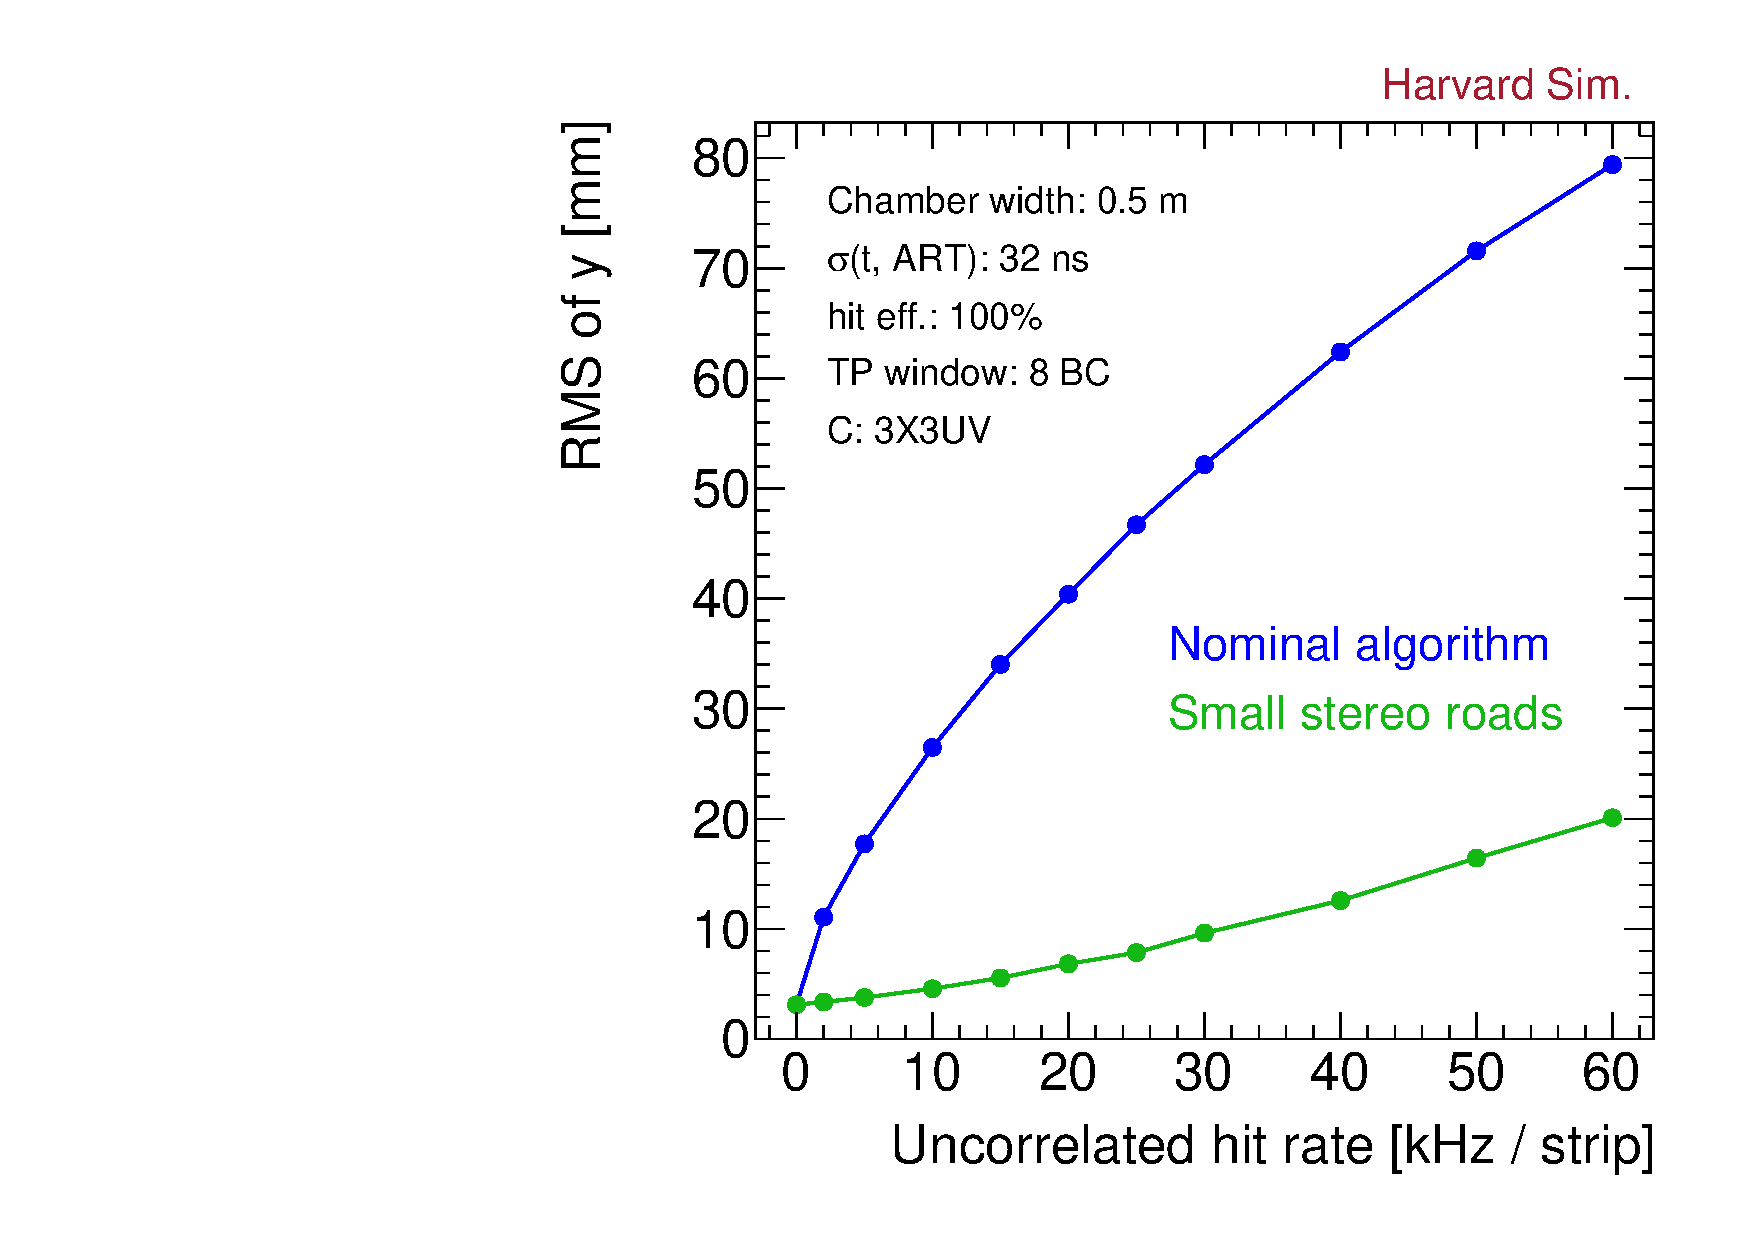
\includegraphics[width=0.48\textwidth]{figures/rms_y_small_vs_rate.pdf}
    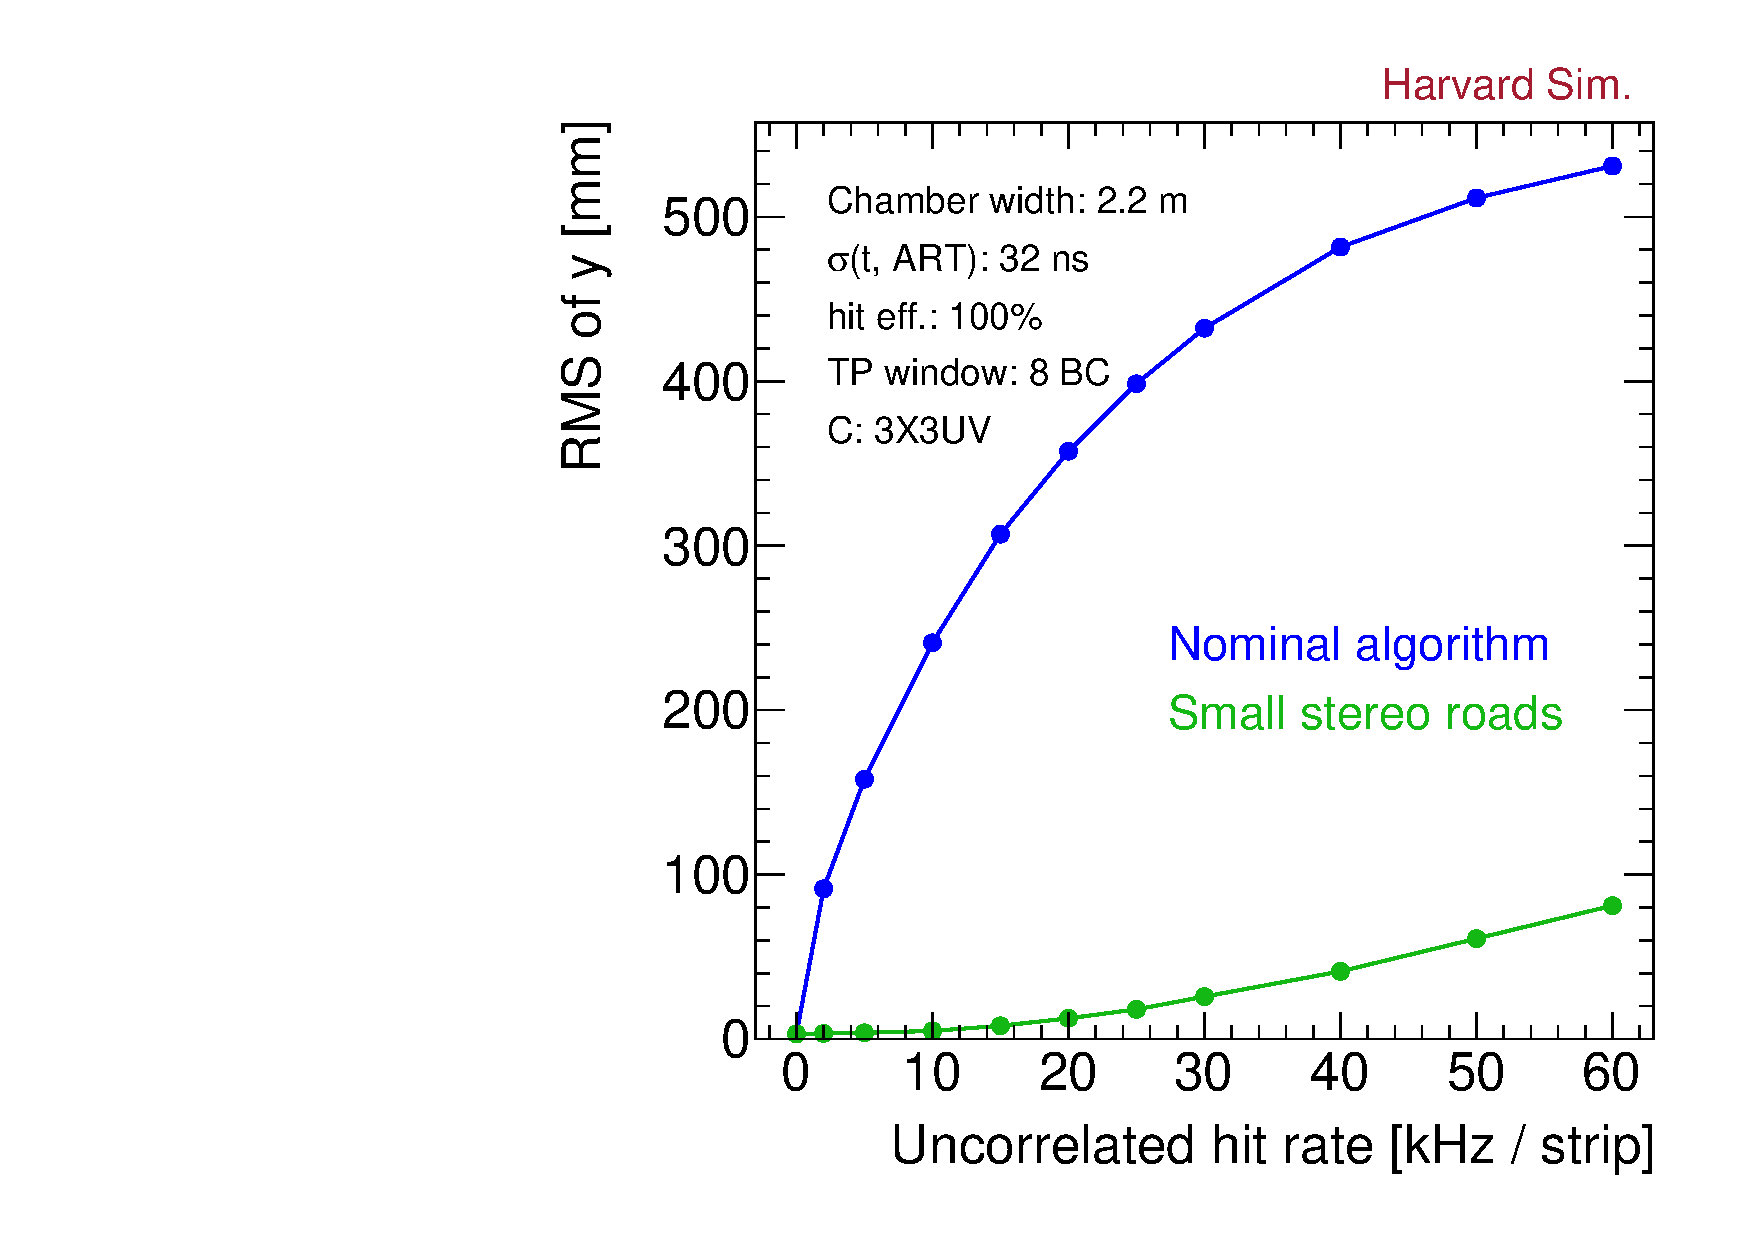
\includegraphics[width=0.48\textwidth]{figures/rms_y_large_vs_rate.pdf}
  \end{center}
  \vspace{-10pt}
  \caption{RMS of $y_\text{reco.} - y_\text{truth}$ for a small chamber of width 0.5m (left) and large chamber of width 2.2m (right) as a function of uncorrelated background rate. The RMS is calculated in the $3\sigma$ (99.7\%) range of the distribution.}
  \label{fig:rms_vs_rate}
\end{figure}

\begin{figure}[!htpb]
  \begin{center}
    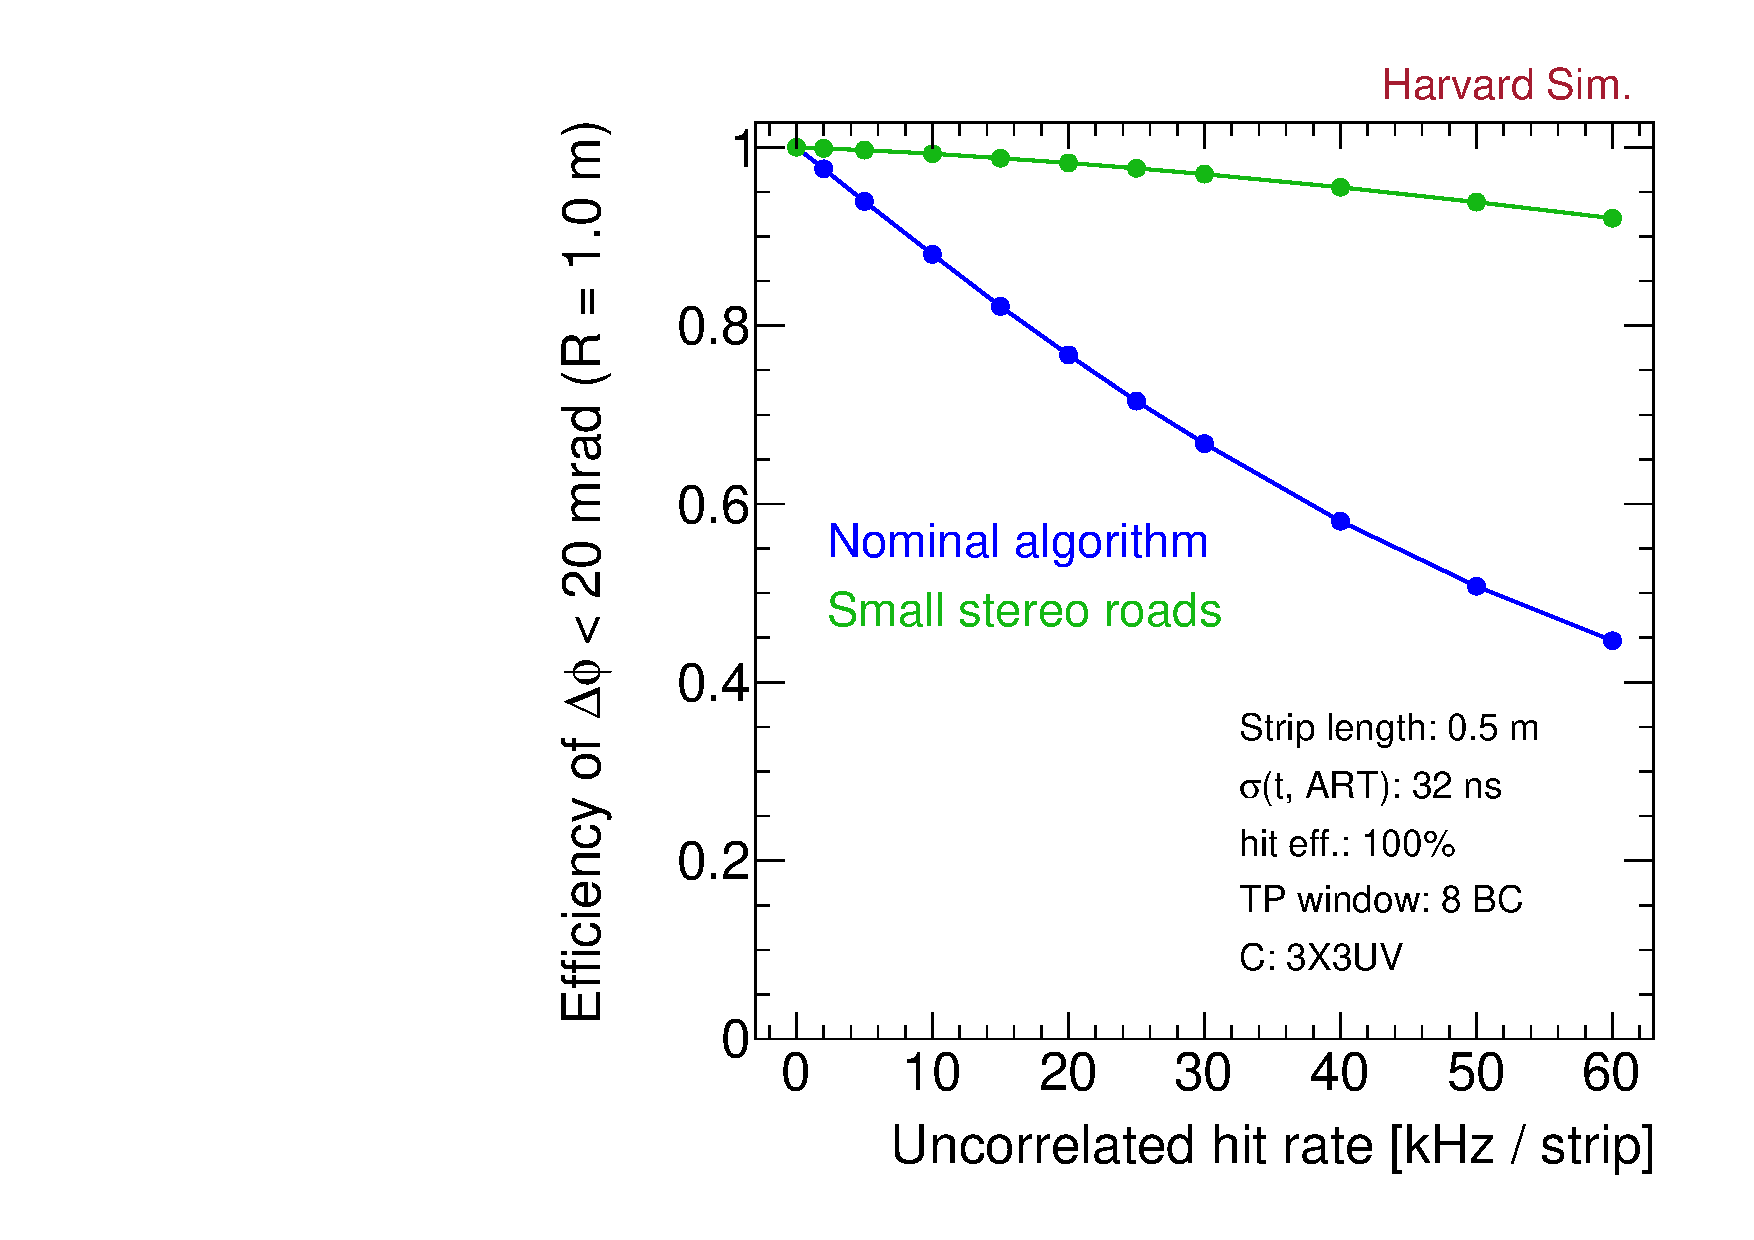
\includegraphics[width=0.48\textwidth]{figures/eff_phi_small_vs_rate.pdf}
    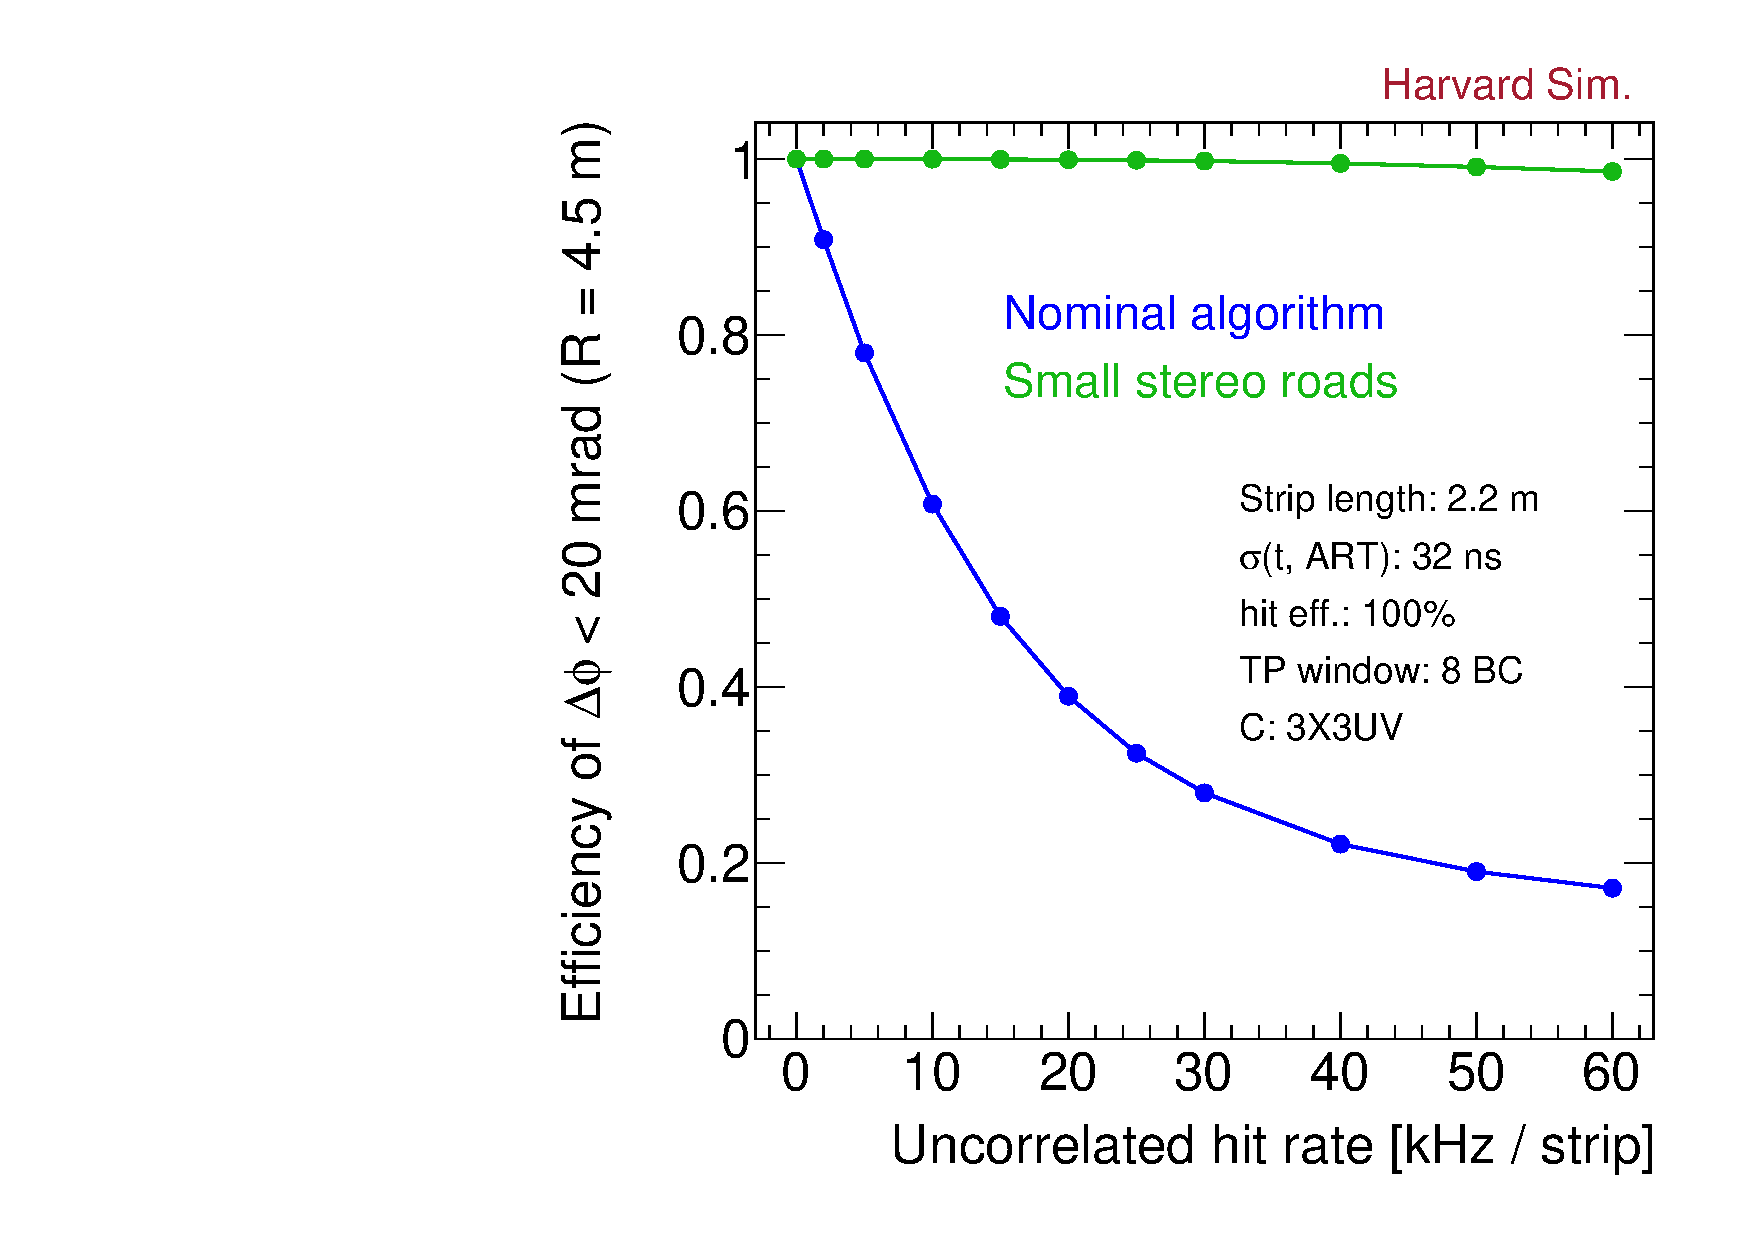
\includegraphics[width=0.48\textwidth]{figures/eff_phi_large_vs_rate.pdf}
  \end{center}
  \vspace{-10pt}
  \caption{Efficiency of $\phi_\text{reco.} - \phi_\text{truth} < 20$ mrad for a small chamber (left) and large chamber (right). $\phi_\text{reco.}-\phi_\text{truth}$ is calculated as $\frac{y_\text{reco.} - y_\text{truth}}{R}$, where $R$ is the distance from the beamline. $R$ is taken to be 1m for the small chamber and 4.5m for the large chamber.}
  \label{fig:eff_vs_rate}
\end{figure}

